\documentclass{article}
\usepackage{amsmath}
\usepackage{graphicx}
\usepackage{../../raccourcis}
\newcommand{\nom}{TD7 : Émission et réception stéréo}
\renewcommand{\nomentete}{UE431 - \nom}

\begin{document}

\titre{\nom}

 Pour transmettre une émission radio en stéréophonie, on code les signaux issus de deux microphones g(t) et d(t) sous la forme :
 \[x_1(t) = (g(t) - d(t)) + \alpha(g(t) - d(t))cos(4\pi f_0t) + A_0cos(2\pi f_0t)\]
 
 Les signaux g(t) et d(t) couvrent une bande de fréquences délimitée par $F_m = 30 Hz$,$F_M = 15kHz$ et $f_0 = 19 kHz$.\\
 
	\noindent 1- $x_1(t)$ peut être réaliser selon le schéma bloc suivant :\\
	\begin{center}
 	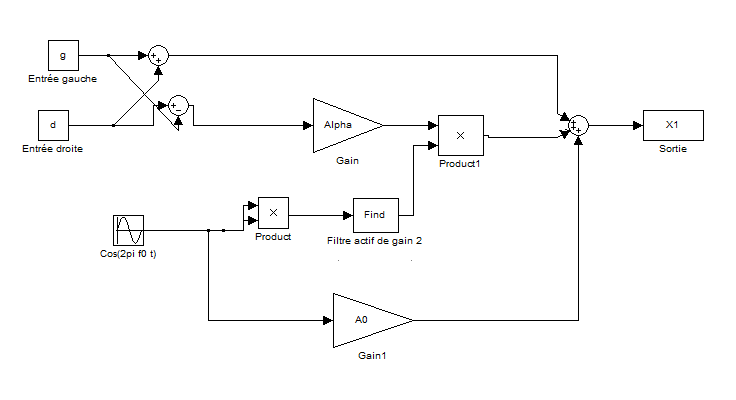
\includegraphics[scale=0.5]{TD7-1.png}
	\end{center}  
 
 	\noindent 2- L'allure du spectre de $x_1$ est la suivante :
 	
 	Il n'y a pas de recouvrement de spectre, $f_0$ étant supérieur à $F_M$.
 	
 	\noindent 3- La bande passante du signal est $B = [F_m ; 2f_0+F_M]$\\
 	
 	\noindent 4- Le but du montage recevant $x_1(t)$ est de restituer $g(t)$ et $d(t)$ sur des voies séparées(stéréo).\\ On considère le montage suivant :
 	
 	\begin{center}
 	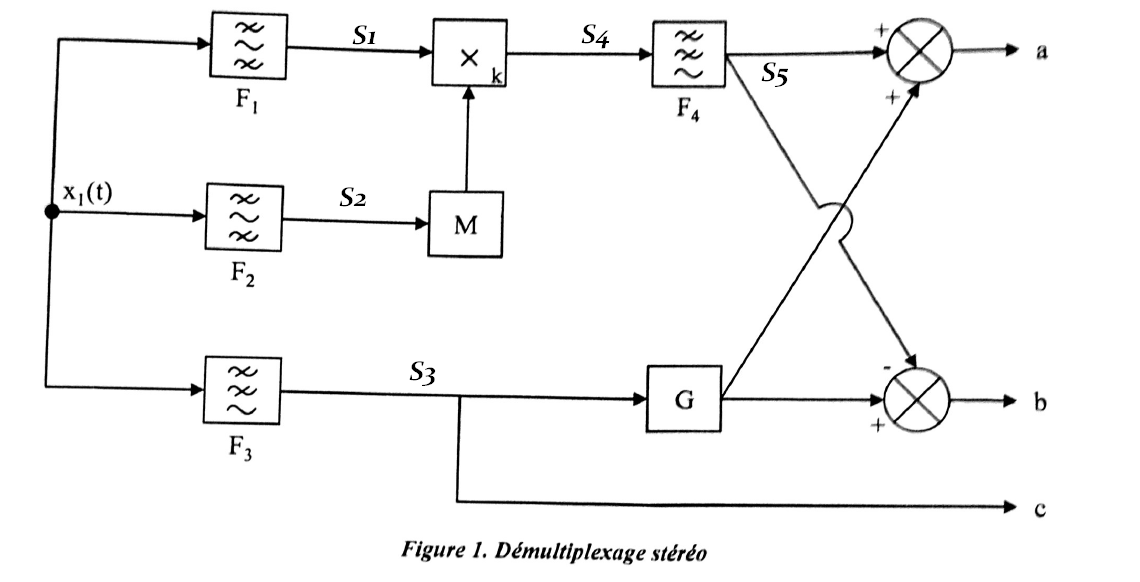
\includegraphics[scale=0.33]{TD7-2.png}
	\end{center}
 	
 	Chaque élément a un rôle propre :\\
 	\begin{itemize}
 	\item M : doubleur(de fréquence)
 	\item G :ampli de gain G
 	\item $F_1$ : filtre passe-bande centré sur $2f_0$
 	\item $F_2$ : filtre passe-bande centré sur $f_0$
 	\item $F_3$ : filtre passe-bas de fréquence de coupure supérieur à $F_m$
 	\item $F_4$ : filtre passe-bas de fréquence de coupure supérieur à $F_m$
 	\end{itemize}
\bigbreak 	
 	
 	Les signaux intérmédiaires sont :\\
 	\begin{itemize}
 	\item $s_1(t) = \alpha (g-d)cos(2\omega_0t)$
 	\item $s_2(t) = A_0 cos(\omega_0t)$
 	\item $s_3(t) = g + d$
 	\item $s_4(t) = k.A_0^2(\frac{1}{2}\alpha (g-d) + \frac{1}{2}\alpha (g-d) cos(4\omega_0t))$
 	\item $s_5(t) = k.A_0^2 \alpha (g-d)$
 	\end{itemize}
\bigbreak 	
 	
 	Déterminons maintenant les sorties :\\
 	\begin{itemize}
 	\item $a = s_5 + G s_3 = k.A_0^2 \alpha.g$ si $G =  \frac{1}{2}k.A_0^2 \alpha$
 	\item $b = G s_3 - s_5 = k.A_0^2 \alpha.d$ si $G =  \frac{1}{2}k.A_0^2 \alpha$
 	\item $c = g+d$
 	\end{itemize}
 	\bigbreak
 	
 	\noindent 5- Réception hétérodyne : on reçoit sur trois canaux centrés respectivement sur $f_{p1}$, $f_{p2}$ et $f_{p3}$ :
 	\[s_n(t) = A_ncos(2\pi f_{pn}t + 2\pi k_f \int_{-\infty}^{t}x_n(t) d\tau)\]
 	
 	Les spectres des signaux en sortie w du multiplieur sont représentés sur la photo suivante :
 	\begin{center}
% 	\includegraphics[scale=0.2]{TD7-3.png}
	\end{center}
	
	Et le zoom pour faire plaisir à l'autre génie :\\
	\begin{center}
 	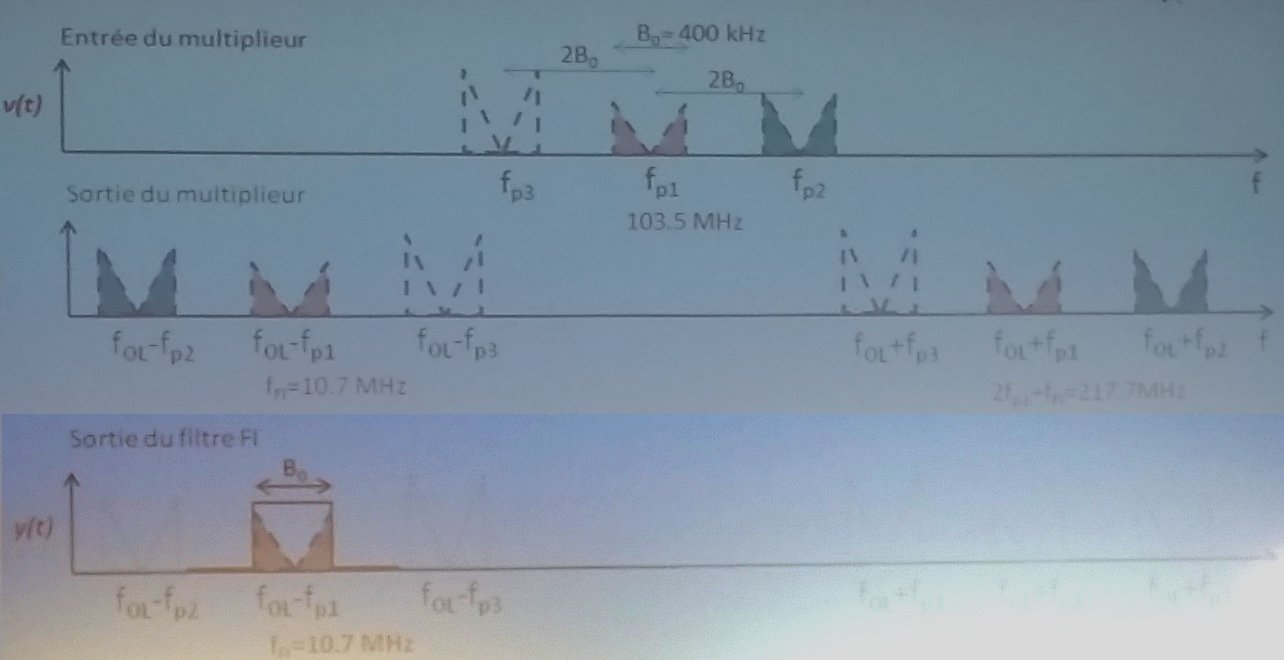
\includegraphics[scale=0.3]{TD7-4.png}
	\end{center}
	
 	
 	\noindent 6- $F_5$ a une bande passante $B_0$ et une fréquence centrale $f_{OL} - f_{p1}$, de sorte que : $Q = \frac{f_{OL} - f_{p1}}{B_0} = \frac{f_{F1}}{B_0} = 26.75$\\
 	Une autre altérnative est de prendre une bande passante $B_0$ et une fréquence centrale $f_{OL} + f_{p1}$ et donc Q = 519 (mais Q est alors trop élevé, et difficile à réaliser).\\
 	
 	\noindent 7- On a $y(t) = A_y cos(2\pi f_{FL}t + 2\pi k_f \int_{-\infty}^{t}x_1(t) d\tau)$ donc le signal FM est constitué de la porteuse de fréquence $f_{F1}$ et l'info est $x_1$\\
 	
 	\noindent 8- En l'absence de multiplieur et d'OL le canal à sélectionner aurait été centré sur $f_{p_1}$. Il aurait fallut un filtre $F_5$ centré sur $f_{p1}$ (très élevé) donc $Q = \frac{f_p}{B_0} >> \frac{f_{FI}}{B}$ et qui plus est accordable(fréquence centrale réglable) donc plus compliqué (WHOOOTT?!!??)\\
 	
 	\noindent 9- On suppose que $f_{FI}$ = 1MHz et qu'on reçoit en plus un signal de porteuse : $f_i = f_{OL} + f_{FI} = f_{p1} + 2f_{FI} = 105.5MHz$\\
 	Dans le récepteur hétérodyne $f_i$ se retrouve multiplié par $f_{OL}$.\\
 	
 	Par conséquent, en sortie de $F_5$ (centrée sur $f_{FI}$) on récupère le transport du signal $f_i$.\\
 	Le problème est que l'on brouille la réception du canal à $f_{p1}$ lui aussi transposé à $f_{FI}$\\
 	
 	$f_i$ est la fréquence image de $f_{P1}$.\\
 	
 	\noindent 10- si $f_{FI} = 10.7MHz$ alors $f_i = f_pi + 2f_{FI} = 114.2MHz$. Donc ce signal est filtré par la bande passante de l'ampli de réception limité a 108MHz. Il n'y a plus de problème.

\end{document}
